\documentclass{whiteboard}
\begin{document}
\begin{frame}[plain,t]
\bbcover{CSES 1750}{Planets Queries I}{Prof. Edson Alves}{Faculdade UnB Gama}

\end{frame}
\begin{frame}[plain,t]
\vspace*{\fill}

\bbenglish{You are playing a game consisting of $n$ planets. Each planet has a teleporter to another planet (or the planet itself).}

\vspace{0.1in}

\bbenglish{Your task is to process $q$ queries of the form: when you begin on planet $x$ and travel through $k$ teleporters, which planet will you reach?}

\vspace*{\fill}
\end{frame}
\begin{frame}[plain,t]
\vspace*{\fill}

\bbtext{Você está jogando um jogo composto de $n$ planetas. Cada planeta tem um teletransporte para outro planeta (ou para si mesmo).}

\vspace{0.1in}

\bbtext{Sua tarefa é processar $q$ consultas da seguinte forma: partindo do planeta $x$ e viajando por $k$ teletransportes, você chegará em qual planeta?}

\vspace*{\fill}
\end{frame}
\begin{frame}[plain,t]
\vspace*{\fill}

\bbbold{Input}

\vspace{0.1in}

\bbenglish{The first input line has two integers $n$ and $q$: the number of planets and queries. The planets are numbered $1, 2, \ldots, n$.}

\vspace{0.1in}

\bbenglish{The second line has $n$ integers $t_1, t_2, \ldots, t_n$: for each planet, the destination of the teleporter. It is possible that $t_i = i$.}

\vspace{0.1in}

\bbenglish{Finally, there are $q$ lines describing the queries. Each line has two integers $x$ and $k$: you start on planet $x$ and travel through $k$ teleporters.}

\vspace{0.2in}

\bbbold{Output}

\vspace{0.1in}

\bbenglish{Print the answer to each query.}

\vspace*{\fill}
\end{frame}
\begin{frame}[plain,t]
\vspace*{\fill}

\bbbold{Entrada}

\vspace{0.1in}

\bbtext{A primeira linha da entrada tem dois inteiros $n$ e $q$: o número de planetas e consultas. Os planetas são numerados $1, 2, \ldots, n$.}

\vspace{0.1in}

\bbtext{A segunda linha contém $n$ inteiros $t_1, t_2, \ldots, t_n$: para cada planeta, o destino do teletransporte. É possível que $t_i = i$.}

\vspace{0.1in}

\bbtext{Finalmente, há $q$ linhas descrevendo as consultas. Cada linha tem dois inteiros $x$ e $k$: você inicia no planeta $x$ e viaja através de $k$ teletransportes.}

\vspace{0.2in}

\bbbold{Saída}

\vspace{0.1in}

\bbtext{Imprima a resposta para cada consulta.}

\vspace*{\fill}
\end{frame}
\begin{frame}[plain,t]
\vspace*{\fill}

\bbbold{Constraints}

\vspace{0.1in}

\begin{itemize}
\item $1\leq n, q\leq 2\times 10^5$
\item $1\leq t_i\leq n$
\item $1\leq x \leq n$
\item $0\leq k\leq 10^9$
\end{itemize}

\vspace*{\fill}
\end{frame}
\begin{frame}[plain,t]
\vspace*{\fill}

\bbbold{Restrições}

\vspace{0.1in}

\begin{itemize}
\item $1\leq n, q\leq 2\times 10^5$
\item $1\leq t_i\leq n$
\item $1\leq x \leq n$
\item $0\leq k\leq 10^9$
\end{itemize}


\vspace*{\fill}
\end{frame}
\begin{frame}[plain,t]
\begin{tikzpicture}
\node[draw,opacity=0] at (0, 0) {x};
\node[draw,opacity=0] at (14, 8) {x};

	\node[anchor=west] (header) at (0, 7.0) { \bbbold{Exemplo de entrada e saída} };

\end{tikzpicture}
\end{frame}
\begin{frame}[plain,t]
\begin{tikzpicture}
\node[draw,opacity=0] at (0, 0) {x};
\node[draw,opacity=0] at (14, 8) {x};

	\node[anchor=west] (header) at (0, 7.0) { \bbbold{Exemplo de entrada e saída} };


	\node[anchor=west] (line1) at (1.0, 6.0) { \bbtext{\texttt{4 3} } };

\end{tikzpicture}
\end{frame}
\begin{frame}[plain,t]
\begin{tikzpicture}
\node[draw,opacity=0] at (0, 0) {x};
\node[draw,opacity=0] at (14, 8) {x};

	\node[anchor=west] (header) at (0, 7.0) { \bbbold{Exemplo de entrada e saída} };


	\node[anchor=west] (line1) at (1.0, 6.0) { \bbtext{\texttt{4 3} } };


	\draw[->,color=BBViolet] (1.25, 5.0) to  (1.25, 5.75);

	\node[] (r) at (1.25, 4.75) { \footnotesize \bbcomment{\# de planetas} };

\end{tikzpicture}
\end{frame}
\begin{frame}[plain,t]
\begin{tikzpicture}
\node[draw,opacity=0] at (0, 0) {x};
\node[draw,opacity=0] at (14, 8) {x};

	\node[anchor=west] (header) at (0, 7.0) { \bbbold{Exemplo de entrada e saída} };


	\node[anchor=west] (line1) at (1.0, 6.0) { \bbtext{\texttt{4 3} } };





	\node[draw,very thick,circle] (node1) at (6.0, 4.0) { \bbtext{1} };

	\node[draw,very thick,circle] (node2) at (8.0, 4.0) { \bbtext{2} };

	\node[draw,very thick,circle] (node3) at (10.0, 4.0) { \bbtext{3} };

	\node[draw,very thick,circle] (node4) at (12.0, 4.0) { \bbtext{4} };

\end{tikzpicture}
\end{frame}
\begin{frame}[plain,t]
\begin{tikzpicture}
\node[draw,opacity=0] at (0, 0) {x};
\node[draw,opacity=0] at (14, 8) {x};

	\node[anchor=west] (header) at (0, 7.0) { \bbbold{Exemplo de entrada e saída} };


	\node[anchor=west] (line1) at (1.0, 6.0) { \bbtext{\texttt{4 3} } };


	\draw[->,color=BBViolet] (1.65, 5.0) to  (1.65, 5.75);

	\node[] (r) at (1.65, 4.75) { \footnotesize \bbcomment{\# de consultas} };


	\node[draw,very thick,circle] (node1) at (6.0, 4.0) { \bbtext{1} };

	\node[draw,very thick,circle] (node2) at (8.0, 4.0) { \bbtext{2} };

	\node[draw,very thick,circle] (node3) at (10.0, 4.0) { \bbtext{3} };

	\node[draw,very thick,circle] (node4) at (12.0, 4.0) { \bbtext{4} };



\end{tikzpicture}
\end{frame}
\begin{frame}[plain,t]
\begin{tikzpicture}
\node[draw,opacity=0] at (0, 0) {x};
\node[draw,opacity=0] at (14, 8) {x};

	\node[anchor=west] (header) at (0, 7.0) { \bbbold{Exemplo de entrada e saída} };


	\node[anchor=west] (line1) at (1.0, 6.0) { \bbtext{\texttt{4 3} } };





	\node[draw,very thick,circle] (node1) at (6.0, 4.0) { \bbtext{1} };

	\node[draw,very thick,circle] (node2) at (8.0, 4.0) { \bbtext{2} };

	\node[draw,very thick,circle] (node3) at (10.0, 4.0) { \bbtext{3} };

	\node[draw,very thick,circle] (node4) at (12.0, 4.0) { \bbtext{4} };




	\node[anchor=west] (line2) at (1.0, 5.5) { \bbtext{\texttt{2 1 1 4} } };

\end{tikzpicture}
\end{frame}
\begin{frame}[plain,t]
\begin{tikzpicture}
\node[draw,opacity=0] at (0, 0) {x};
\node[draw,opacity=0] at (14, 8) {x};

	\node[anchor=west] (header) at (0, 7.0) { \bbbold{Exemplo de entrada e saída} };


	\node[anchor=west] (line1) at (1.0, 6.0) { \bbtext{\texttt{4 3} } };


	\draw[->,color=BBViolet] (1.25, 4.5) to  (1.25, 5.25);

	\node[] (r) at (1.25, 4.25) { $t_1$ };


	\node[draw,very thick,circle] (node1) at (6.0, 4.0) { \bbtext{1} };

	\node[draw,very thick,circle] (node2) at (8.0, 4.0) { \bbtext{2} };

	\node[draw,very thick,circle] (node3) at (10.0, 4.0) { \bbtext{3} };

	\node[draw,very thick,circle] (node4) at (12.0, 4.0) { \bbtext{4} };




	\node[anchor=west] (line2) at (1.0, 5.5) { \bbtext{\texttt{2 1 1 4} } };



\end{tikzpicture}
\end{frame}
\begin{frame}[plain,t]
\begin{tikzpicture}
\node[draw,opacity=0] at (0, 0) {x};
\node[draw,opacity=0] at (14, 8) {x};

	\node[anchor=west] (header) at (0, 7.0) { \bbbold{Exemplo de entrada e saída} };


	\node[anchor=west] (line1) at (1.0, 6.0) { \bbtext{\texttt{4 3} } };


	\draw[->,color=BBViolet] (1.25, 4.5) to  (1.25, 5.25);

	\node[] (r) at (1.25, 4.25) { $t_1$ };


	\node[draw,very thick,circle] (node1) at (6.0, 4.0) { \bbtext{1} };

	\node[draw,very thick,circle] (node2) at (8.0, 4.0) { \bbtext{2} };

	\node[draw,very thick,circle] (node3) at (10.0, 4.0) { \bbtext{3} };

	\node[draw,very thick,circle] (node4) at (12.0, 4.0) { \bbtext{4} };




	\node[anchor=west] (line2) at (1.0, 5.5) { \bbtext{\texttt{2 1 1 4} } };




	\draw[thick,-latex](node1) to (node2);

\end{tikzpicture}
\end{frame}
\begin{frame}[plain,t]
\begin{tikzpicture}
\node[draw,opacity=0] at (0, 0) {x};
\node[draw,opacity=0] at (14, 8) {x};

	\node[anchor=west] (header) at (0, 7.0) { \bbbold{Exemplo de entrada e saída} };


	\node[anchor=west] (line1) at (1.0, 6.0) { \bbtext{\texttt{4 3} } };


	\draw[->,color=BBViolet] (1.65, 4.5) to  (1.65, 5.25);

	\node[] (r) at (1.65, 4.25) { $t_2$ };


	\node[draw,very thick,circle] (node1) at (6.0, 4.0) { \bbtext{1} };

	\node[draw,very thick,circle] (node2) at (8.0, 4.0) { \bbtext{2} };

	\node[draw,very thick,circle] (node3) at (10.0, 4.0) { \bbtext{3} };

	\node[draw,very thick,circle] (node4) at (12.0, 4.0) { \bbtext{4} };




	\node[anchor=west] (line2) at (1.0, 5.5) { \bbtext{\texttt{2 1 1 4} } };




	\draw[thick,-latex](node1) to (node2);



\end{tikzpicture}
\end{frame}
\begin{frame}[plain,t]
\begin{tikzpicture}
\node[draw,opacity=0] at (0, 0) {x};
\node[draw,opacity=0] at (14, 8) {x};

	\node[anchor=west] (header) at (0, 7.0) { \bbbold{Exemplo de entrada e saída} };


	\node[anchor=west] (line1) at (1.0, 6.0) { \bbtext{\texttt{4 3} } };


	\draw[->,color=BBViolet] (1.65, 4.5) to  (1.65, 5.25);

	\node[] (r) at (1.65, 4.25) { $t_2$ };


	\node[draw,very thick,circle] (node1) at (6.0, 4.0) { \bbtext{1} };

	\node[draw,very thick,circle] (node2) at (8.0, 4.0) { \bbtext{2} };

	\node[draw,very thick,circle] (node3) at (10.0, 4.0) { \bbtext{3} };

	\node[draw,very thick,circle] (node4) at (12.0, 4.0) { \bbtext{4} };




	\node[anchor=west] (line2) at (1.0, 5.5) { \bbtext{\texttt{2 1 1 4} } };




	\draw[thick,-latex](node1) to (node2);




	\draw[thick,-latex](node2) to [bend right] (node1);

\end{tikzpicture}
\end{frame}
\begin{frame}[plain,t]
\begin{tikzpicture}
\node[draw,opacity=0] at (0, 0) {x};
\node[draw,opacity=0] at (14, 8) {x};

	\node[anchor=west] (header) at (0, 7.0) { \bbbold{Exemplo de entrada e saída} };


	\node[anchor=west] (line1) at (1.0, 6.0) { \bbtext{\texttt{4 3} } };


	\draw[->,color=BBViolet] (2.05, 4.5) to  (2.05, 5.25);

	\node[] (r) at (2.05, 4.25) { $t_3$ };


	\node[draw,very thick,circle] (node1) at (6.0, 4.0) { \bbtext{1} };

	\node[draw,very thick,circle] (node2) at (8.0, 4.0) { \bbtext{2} };

	\node[draw,very thick,circle] (node3) at (10.0, 4.0) { \bbtext{3} };

	\node[draw,very thick,circle] (node4) at (12.0, 4.0) { \bbtext{4} };




	\node[anchor=west] (line2) at (1.0, 5.5) { \bbtext{\texttt{2 1 1 4} } };




	\draw[thick,-latex](node1) to (node2);




	\draw[thick,-latex](node2) to [bend right] (node1);



\end{tikzpicture}
\end{frame}
\begin{frame}[plain,t]
\begin{tikzpicture}
\node[draw,opacity=0] at (0, 0) {x};
\node[draw,opacity=0] at (14, 8) {x};

	\node[anchor=west] (header) at (0, 7.0) { \bbbold{Exemplo de entrada e saída} };


	\node[anchor=west] (line1) at (1.0, 6.0) { \bbtext{\texttt{4 3} } };


	\draw[->,color=BBViolet] (2.05, 4.5) to  (2.05, 5.25);

	\node[] (r) at (2.05, 4.25) { $t_3$ };


	\node[draw,very thick,circle] (node1) at (6.0, 4.0) { \bbtext{1} };

	\node[draw,very thick,circle] (node2) at (8.0, 4.0) { \bbtext{2} };

	\node[draw,very thick,circle] (node3) at (10.0, 4.0) { \bbtext{3} };

	\node[draw,very thick,circle] (node4) at (12.0, 4.0) { \bbtext{4} };




	\node[anchor=west] (line2) at (1.0, 5.5) { \bbtext{\texttt{2 1 1 4} } };




	\draw[thick,-latex](node1) to (node2);




	\draw[thick,-latex](node2) to [bend right] (node1);




	\draw[thick,-latex](node3) to [bend left] (node1);

\end{tikzpicture}
\end{frame}
\begin{frame}[plain,t]
\begin{tikzpicture}
\node[draw,opacity=0] at (0, 0) {x};
\node[draw,opacity=0] at (14, 8) {x};

	\node[anchor=west] (header) at (0, 7.0) { \bbbold{Exemplo de entrada e saída} };


	\node[anchor=west] (line1) at (1.0, 6.0) { \bbtext{\texttt{4 3} } };


	\draw[->,color=BBViolet] (2.45, 4.5) to  (2.45, 5.25);

	\node[] (r) at (2.45, 4.25) { $t_4$ };


	\node[draw,very thick,circle] (node1) at (6.0, 4.0) { \bbtext{1} };

	\node[draw,very thick,circle] (node2) at (8.0, 4.0) { \bbtext{2} };

	\node[draw,very thick,circle] (node3) at (10.0, 4.0) { \bbtext{3} };

	\node[draw,very thick,circle] (node4) at (12.0, 4.0) { \bbtext{4} };




	\node[anchor=west] (line2) at (1.0, 5.5) { \bbtext{\texttt{2 1 1 4} } };




	\draw[thick,-latex](node1) to (node2);




	\draw[thick,-latex](node2) to [bend right] (node1);




	\draw[thick,-latex](node3) to [bend left] (node1);



\end{tikzpicture}
\end{frame}
\begin{frame}[plain,t]
\begin{tikzpicture}
\node[draw,opacity=0] at (0, 0) {x};
\node[draw,opacity=0] at (14, 8) {x};

	\node[anchor=west] (header) at (0, 7.0) { \bbbold{Exemplo de entrada e saída} };


	\node[anchor=west] (line1) at (1.0, 6.0) { \bbtext{\texttt{4 3} } };


	\draw[->,color=BBViolet] (2.45, 4.5) to  (2.45, 5.25);

	\node[] (r) at (2.45, 4.25) { $t_4$ };


	\node[draw,very thick,circle] (node1) at (6.0, 4.0) { \bbtext{1} };

	\node[draw,very thick,circle] (node2) at (8.0, 4.0) { \bbtext{2} };

	\node[draw,very thick,circle] (node3) at (10.0, 4.0) { \bbtext{3} };

	\node[draw,very thick,circle] (node4) at (12.0, 4.0) { \bbtext{4} };




	\node[anchor=west] (line2) at (1.0, 5.5) { \bbtext{\texttt{2 1 1 4} } };




	\draw[thick,-latex](node1) to (node2);




	\draw[thick,-latex](node2) to [bend right] (node1);




	\draw[thick,-latex](node3) to [bend left] (node1);




	\draw[thick,-latex](node4) to [loop right] (node4);

\end{tikzpicture}
\end{frame}
\begin{frame}[plain,t]
\begin{tikzpicture}
\node[draw,opacity=0] at (0, 0) {x};
\node[draw,opacity=0] at (14, 8) {x};

	\node[anchor=west] (header) at (0, 7.0) { \bbbold{Exemplo de entrada e saída} };


	\node[anchor=west] (line1) at (1.0, 6.0) { \bbtext{\texttt{4 3} } };





	\node[draw,very thick,circle] (node1) at (6.0, 4.0) { \bbtext{1} };

	\node[draw,very thick,circle] (node2) at (8.0, 4.0) { \bbtext{2} };

	\node[draw,very thick,circle] (node3) at (10.0, 4.0) { \bbtext{3} };

	\node[draw,very thick,circle] (node4) at (12.0, 4.0) { \bbtext{4} };




	\node[anchor=west] (line2) at (1.0, 5.5) { \bbtext{\texttt{2 1 1 4} } };




	\draw[thick,-latex](node1) to (node2);




	\draw[thick,-latex](node2) to [bend right] (node1);




	\draw[thick,-latex](node3) to [bend left] (node1);




	\draw[thick,-latex](node4) to [loop right] (node4);



	\node[anchor=west] (line3) at (1.0, 5.0) { \bbtext{\texttt{1 2} } };

\end{tikzpicture}
\end{frame}
\begin{frame}[plain,t]
\begin{tikzpicture}
\node[draw,opacity=0] at (0, 0) {x};
\node[draw,opacity=0] at (14, 8) {x};

	\node[anchor=west] (header) at (0, 7.0) { \bbbold{Exemplo de entrada e saída} };


	\node[anchor=west] (line1) at (1.0, 6.0) { \bbtext{\texttt{4 3} } };


	\draw[->,color=BBViolet] (1.25, 4.0) to  (1.25, 4.75);

	\node[] (r) at (1.25, 3.75) { $x$ };


	\node[draw,very thick,circle] (node1) at (6.0, 4.0) { \bbtext{1} };

	\node[draw,very thick,circle] (node2) at (8.0, 4.0) { \bbtext{2} };

	\node[draw,very thick,circle] (node3) at (10.0, 4.0) { \bbtext{3} };

	\node[draw,very thick,circle] (node4) at (12.0, 4.0) { \bbtext{4} };




	\node[anchor=west] (line2) at (1.0, 5.5) { \bbtext{\texttt{2 1 1 4} } };




	\draw[thick,-latex](node1) to (node2);




	\draw[thick,-latex](node2) to [bend right] (node1);




	\draw[thick,-latex](node3) to [bend left] (node1);




	\draw[thick,-latex](node4) to [loop right] (node4);



	\node[anchor=west] (line3) at (1.0, 5.0) { \bbtext{\texttt{1 2} } };



\end{tikzpicture}
\end{frame}
\begin{frame}[plain,t]
\begin{tikzpicture}
\node[draw,opacity=0] at (0, 0) {x};
\node[draw,opacity=0] at (14, 8) {x};

	\node[anchor=west] (header) at (0, 7.0) { \bbbold{Exemplo de entrada e saída} };


	\node[anchor=west] (line1) at (1.0, 6.0) { \bbtext{\texttt{4 3} } };


	\draw[->,color=BBViolet] (1.25, 4.0) to  (1.25, 4.75);

	\node[] (r) at (1.25, 3.75) { $x$ };


	\node[draw,very thick,circle,fill=BBGreen] (node1) at (6.0, 4.0) { \bbtext{1} };

	\node[draw,very thick,circle] (node2) at (8.0, 4.0) { \bbtext{2} };

	\node[draw,very thick,circle] (node3) at (10.0, 4.0) { \bbtext{3} };

	\node[draw,very thick,circle] (node4) at (12.0, 4.0) { \bbtext{4} };




	\node[anchor=west] (line2) at (1.0, 5.5) { \bbtext{\texttt{2 1 1 4} } };




	\draw[thick,-latex](node1) to (node2);




	\draw[thick,-latex](node2) to [bend right] (node1);




	\draw[thick,-latex](node3) to [bend left] (node1);




	\draw[thick,-latex](node4) to [loop right] (node4);



	\node[anchor=west] (line3) at (1.0, 5.0) { \bbtext{\texttt{1 2} } };




\end{tikzpicture}
\end{frame}
\begin{frame}[plain,t]
\begin{tikzpicture}
\node[draw,opacity=0] at (0, 0) {x};
\node[draw,opacity=0] at (14, 8) {x};

	\node[anchor=west] (header) at (0, 7.0) { \bbbold{Exemplo de entrada e saída} };


	\node[anchor=west] (line1) at (1.0, 6.0) { \bbtext{\texttt{4 3} } };


	\draw[->,color=BBViolet] (1.65, 4.0) to  (1.65, 4.75);

	\node[] (r) at (1.65, 3.75) { $k$ };


	\node[draw,very thick,circle,fill=BBGreen] (node1) at (6.0, 4.0) { \bbtext{1} };

	\node[draw,very thick,circle] (node2) at (8.0, 4.0) { \bbtext{2} };

	\node[draw,very thick,circle] (node3) at (10.0, 4.0) { \bbtext{3} };

	\node[draw,very thick,circle] (node4) at (12.0, 4.0) { \bbtext{4} };




	\node[anchor=west] (line2) at (1.0, 5.5) { \bbtext{\texttt{2 1 1 4} } };




	\draw[thick,-latex](node1) to (node2);




	\draw[thick,-latex](node2) to [bend right] (node1);




	\draw[thick,-latex](node3) to [bend left] (node1);




	\draw[thick,-latex](node4) to [loop right] (node4);



	\node[anchor=west] (line3) at (1.0, 5.0) { \bbtext{\texttt{1 2} } };






\end{tikzpicture}
\end{frame}
\begin{frame}[plain,t]
\begin{tikzpicture}
\node[draw,opacity=0] at (0, 0) {x};
\node[draw,opacity=0] at (14, 8) {x};

	\node[anchor=west] (header) at (0, 7.0) { \bbbold{Exemplo de entrada e saída} };


	\node[anchor=west] (line1) at (1.0, 6.0) { \bbtext{\texttt{4 3} } };





	\node[draw,very thick,circle,fill=BBGreen] (node1) at (6.0, 4.0) { \bbtext{1} };

	\node[draw,very thick,circle,fill=BBOrange] (node2) at (8.0, 4.0) { \bbtext{2} };

	\node[draw,very thick,circle] (node3) at (10.0, 4.0) { \bbtext{3} };

	\node[draw,very thick,circle] (node4) at (12.0, 4.0) { \bbtext{4} };




	\node[anchor=west] (line2) at (1.0, 5.5) { \bbtext{\texttt{2 1 1 4} } };




	\draw[thick,-latex](node1) to (node2);




	\draw[thick,-latex](node2) to [bend right] (node1);




	\draw[thick,-latex](node3) to [bend left] (node1);




	\draw[thick,-latex](node4) to [loop right] (node4);



	\node[anchor=west] (line3) at (1.0, 5.0) { \bbtext{\texttt{1 2} } };








\end{tikzpicture}
\end{frame}
\begin{frame}[plain,t]
\begin{tikzpicture}
\node[draw,opacity=0] at (0, 0) {x};
\node[draw,opacity=0] at (14, 8) {x};

	\node[anchor=west] (header) at (0, 7.0) { \bbbold{Exemplo de entrada e saída} };


	\node[anchor=west] (line1) at (1.0, 6.0) { \bbtext{\texttt{4 3} } };





	\node[draw,very thick,circle,fill=BBCyan] (node1) at (6.0, 4.0) { \bbtext{1} };

	\node[draw,very thick,circle,fill=BBWhite] (node2) at (8.0, 4.0) { \bbtext{2} };

	\node[draw,very thick,circle] (node3) at (10.0, 4.0) { \bbtext{3} };

	\node[draw,very thick,circle] (node4) at (12.0, 4.0) { \bbtext{4} };




	\node[anchor=west] (line2) at (1.0, 5.5) { \bbtext{\texttt{2 1 1 4} } };




	\draw[thick,-latex](node1) to (node2);




	\draw[thick,-latex](node2) to [bend right] (node1);




	\draw[thick,-latex](node3) to [bend left] (node1);




	\draw[thick,-latex](node4) to [loop right] (node4);



	\node[anchor=west] (line3) at (1.0, 5.0) { \bbtext{\texttt{1 2} } };









\end{tikzpicture}
\end{frame}
\begin{frame}[plain,t]
\begin{tikzpicture}
\node[draw,opacity=0] at (0, 0) {x};
\node[draw,opacity=0] at (14, 8) {x};

	\node[anchor=west] (header) at (0, 7.0) { \bbbold{Exemplo de entrada e saída} };


	\node[anchor=west] (line1) at (1.0, 6.0) { \bbtext{\texttt{4 3} } };


	\draw[->,color=BBBlack,thick,-latex] (2.0, 5.0) to  (3.0, 5.0);

	\node[anchor=west] (r) at (3.0, 5.0) { \footnotesize \bboutput{1} };


	\node[draw,very thick,circle,fill=BBCyan] (node1) at (6.0, 4.0) { \bbtext{1} };

	\node[draw,very thick,circle,fill=BBWhite] (node2) at (8.0, 4.0) { \bbtext{2} };

	\node[draw,very thick,circle] (node3) at (10.0, 4.0) { \bbtext{3} };

	\node[draw,very thick,circle] (node4) at (12.0, 4.0) { \bbtext{4} };




	\node[anchor=west] (line2) at (1.0, 5.5) { \bbtext{\texttt{2 1 1 4} } };




	\draw[thick,-latex](node1) to (node2);




	\draw[thick,-latex](node2) to [bend right] (node1);




	\draw[thick,-latex](node3) to [bend left] (node1);




	\draw[thick,-latex](node4) to [loop right] (node4);



	\node[anchor=west] (line3) at (1.0, 5.0) { \bbtext{\texttt{1 2} } };











\end{tikzpicture}
\end{frame}
\begin{frame}[plain,t]
\begin{tikzpicture}
\node[draw,opacity=0] at (0, 0) {x};
\node[draw,opacity=0] at (14, 8) {x};

	\node[anchor=west] (header) at (0, 7.0) { \bbbold{Exemplo de entrada e saída} };


	\node[anchor=west] (line1) at (1.0, 6.0) { \bbtext{\texttt{4 3} } };





	\node[draw,very thick,circle,fill=BBWhite] (node1) at (6.0, 4.0) { \bbtext{1} };

	\node[draw,very thick,circle,fill=BBWhite] (node2) at (8.0, 4.0) { \bbtext{2} };

	\node[draw,very thick,circle] (node3) at (10.0, 4.0) { \bbtext{3} };

	\node[draw,very thick,circle] (node4) at (12.0, 4.0) { \bbtext{4} };




	\node[anchor=west] (line2) at (1.0, 5.5) { \bbtext{\texttt{2 1 1 4} } };




	\draw[thick,-latex](node1) to (node2);




	\draw[thick,-latex](node2) to [bend right] (node1);




	\draw[thick,-latex](node3) to [bend left] (node1);




	\draw[thick,-latex](node4) to [loop right] (node4);



	\node[anchor=west] (line3) at (1.0, 5.0) { \bbtext{\texttt{1 2} } };














	\node[anchor=west] (line4) at (1.0, 4.5) { \bbtext{\texttt{3 4} } };

\end{tikzpicture}
\end{frame}
\begin{frame}[plain,t]
\begin{tikzpicture}
\node[draw,opacity=0] at (0, 0) {x};
\node[draw,opacity=0] at (14, 8) {x};

	\node[anchor=west] (header) at (0, 7.0) { \bbbold{Exemplo de entrada e saída} };


	\node[anchor=west] (line1) at (1.0, 6.0) { \bbtext{\texttt{4 3} } };





	\node[draw,very thick,circle,fill=BBWhite] (node1) at (6.0, 4.0) { \bbtext{1} };

	\node[draw,very thick,circle,fill=BBWhite] (node2) at (8.0, 4.0) { \bbtext{2} };

	\node[draw,very thick,circle,fill=BBGreen] (node3) at (10.0, 4.0) { \bbtext{3} };

	\node[draw,very thick,circle] (node4) at (12.0, 4.0) { \bbtext{4} };




	\node[anchor=west] (line2) at (1.0, 5.5) { \bbtext{\texttt{2 1 1 4} } };




	\draw[thick,-latex](node1) to (node2);




	\draw[thick,-latex](node2) to [bend right] (node1);




	\draw[thick,-latex](node3) to [bend left] (node1);




	\draw[thick,-latex](node4) to [loop right] (node4);



	\node[anchor=west] (line3) at (1.0, 5.0) { \bbtext{\texttt{1 2} } };














	\node[anchor=west] (line4) at (1.0, 4.5) { \bbtext{\texttt{3 4} } };


\end{tikzpicture}
\end{frame}
\begin{frame}[plain,t]
\begin{tikzpicture}
\node[draw,opacity=0] at (0, 0) {x};
\node[draw,opacity=0] at (14, 8) {x};

	\node[anchor=west] (header) at (0, 7.0) { \bbbold{Exemplo de entrada e saída} };


	\node[anchor=west] (line1) at (1.0, 6.0) { \bbtext{\texttt{4 3} } };





	\node[draw,very thick,circle,fill=BBOrange] (node1) at (6.0, 4.0) { \bbtext{1} };

	\node[draw,very thick,circle,fill=BBWhite] (node2) at (8.0, 4.0) { \bbtext{2} };

	\node[draw,very thick,circle,fill=BBGreen] (node3) at (10.0, 4.0) { \bbtext{3} };

	\node[draw,very thick,circle] (node4) at (12.0, 4.0) { \bbtext{4} };




	\node[anchor=west] (line2) at (1.0, 5.5) { \bbtext{\texttt{2 1 1 4} } };




	\draw[thick,-latex](node1) to (node2);




	\draw[thick,-latex](node2) to [bend right] (node1);




	\draw[thick,-latex](node3) to [bend left] (node1);




	\draw[thick,-latex](node4) to [loop right] (node4);



	\node[anchor=west] (line3) at (1.0, 5.0) { \bbtext{\texttt{1 2} } };














	\node[anchor=west] (line4) at (1.0, 4.5) { \bbtext{\texttt{3 4} } };


\end{tikzpicture}
\end{frame}
\begin{frame}[plain,t]
\begin{tikzpicture}
\node[draw,opacity=0] at (0, 0) {x};
\node[draw,opacity=0] at (14, 8) {x};

	\node[anchor=west] (header) at (0, 7.0) { \bbbold{Exemplo de entrada e saída} };


	\node[anchor=west] (line1) at (1.0, 6.0) { \bbtext{\texttt{4 3} } };





	\node[draw,very thick,circle,fill=BBWhite] (node1) at (6.0, 4.0) { \bbtext{1} };

	\node[draw,very thick,circle,fill=BBOrange] (node2) at (8.0, 4.0) { \bbtext{2} };

	\node[draw,very thick,circle,fill=BBGreen] (node3) at (10.0, 4.0) { \bbtext{3} };

	\node[draw,very thick,circle] (node4) at (12.0, 4.0) { \bbtext{4} };




	\node[anchor=west] (line2) at (1.0, 5.5) { \bbtext{\texttt{2 1 1 4} } };




	\draw[thick,-latex](node1) to (node2);




	\draw[thick,-latex](node2) to [bend right] (node1);




	\draw[thick,-latex](node3) to [bend left] (node1);




	\draw[thick,-latex](node4) to [loop right] (node4);



	\node[anchor=west] (line3) at (1.0, 5.0) { \bbtext{\texttt{1 2} } };














	\node[anchor=west] (line4) at (1.0, 4.5) { \bbtext{\texttt{3 4} } };


\end{tikzpicture}
\end{frame}
\begin{frame}[plain,t]
\begin{tikzpicture}
\node[draw,opacity=0] at (0, 0) {x};
\node[draw,opacity=0] at (14, 8) {x};

	\node[anchor=west] (header) at (0, 7.0) { \bbbold{Exemplo de entrada e saída} };


	\node[anchor=west] (line1) at (1.0, 6.0) { \bbtext{\texttt{4 3} } };





	\node[draw,very thick,circle,fill=BBOrange] (node1) at (6.0, 4.0) { \bbtext{1} };

	\node[draw,very thick,circle,fill=BBWhite] (node2) at (8.0, 4.0) { \bbtext{2} };

	\node[draw,very thick,circle,fill=BBGreen] (node3) at (10.0, 4.0) { \bbtext{3} };

	\node[draw,very thick,circle] (node4) at (12.0, 4.0) { \bbtext{4} };




	\node[anchor=west] (line2) at (1.0, 5.5) { \bbtext{\texttt{2 1 1 4} } };




	\draw[thick,-latex](node1) to (node2);




	\draw[thick,-latex](node2) to [bend right] (node1);




	\draw[thick,-latex](node3) to [bend left] (node1);




	\draw[thick,-latex](node4) to [loop right] (node4);



	\node[anchor=west] (line3) at (1.0, 5.0) { \bbtext{\texttt{1 2} } };














	\node[anchor=west] (line4) at (1.0, 4.5) { \bbtext{\texttt{3 4} } };


\end{tikzpicture}
\end{frame}
\begin{frame}[plain,t]
\begin{tikzpicture}
\node[draw,opacity=0] at (0, 0) {x};
\node[draw,opacity=0] at (14, 8) {x};

	\node[anchor=west] (header) at (0, 7.0) { \bbbold{Exemplo de entrada e saída} };


	\node[anchor=west] (line1) at (1.0, 6.0) { \bbtext{\texttt{4 3} } };





	\node[draw,very thick,circle,fill=BBWhite] (node1) at (6.0, 4.0) { \bbtext{1} };

	\node[draw,very thick,circle,fill=BBCyan] (node2) at (8.0, 4.0) { \bbtext{2} };

	\node[draw,very thick,circle,fill=BBGreen] (node3) at (10.0, 4.0) { \bbtext{3} };

	\node[draw,very thick,circle] (node4) at (12.0, 4.0) { \bbtext{4} };




	\node[anchor=west] (line2) at (1.0, 5.5) { \bbtext{\texttt{2 1 1 4} } };




	\draw[thick,-latex](node1) to (node2);




	\draw[thick,-latex](node2) to [bend right] (node1);




	\draw[thick,-latex](node3) to [bend left] (node1);




	\draw[thick,-latex](node4) to [loop right] (node4);



	\node[anchor=west] (line3) at (1.0, 5.0) { \bbtext{\texttt{1 2} } };














	\node[anchor=west] (line4) at (1.0, 4.5) { \bbtext{\texttt{3 4} } };



\end{tikzpicture}
\end{frame}
\begin{frame}[plain,t]
\begin{tikzpicture}
\node[draw,opacity=0] at (0, 0) {x};
\node[draw,opacity=0] at (14, 8) {x};

	\node[anchor=west] (header) at (0, 7.0) { \bbbold{Exemplo de entrada e saída} };


	\node[anchor=west] (line1) at (1.0, 6.0) { \bbtext{\texttt{4 3} } };


	\draw[->,color=BBBlack,thick,-latex] (2.0, 4.5) to  (3.0, 4.5);

	\node[anchor=west] (r) at (3.0, 4.5) { \footnotesize \bboutput{2} };


	\node[draw,very thick,circle,fill=BBWhite] (node1) at (6.0, 4.0) { \bbtext{1} };

	\node[draw,very thick,circle,fill=BBCyan] (node2) at (8.0, 4.0) { \bbtext{2} };

	\node[draw,very thick,circle,fill=BBGreen] (node3) at (10.0, 4.0) { \bbtext{3} };

	\node[draw,very thick,circle] (node4) at (12.0, 4.0) { \bbtext{4} };




	\node[anchor=west] (line2) at (1.0, 5.5) { \bbtext{\texttt{2 1 1 4} } };




	\draw[thick,-latex](node1) to (node2);




	\draw[thick,-latex](node2) to [bend right] (node1);




	\draw[thick,-latex](node3) to [bend left] (node1);




	\draw[thick,-latex](node4) to [loop right] (node4);



	\node[anchor=west] (line3) at (1.0, 5.0) { \bbtext{\texttt{1 2} } };














	\node[anchor=west] (line4) at (1.0, 4.5) { \bbtext{\texttt{3 4} } };





\end{tikzpicture}
\end{frame}
\begin{frame}[plain,t]
\begin{tikzpicture}
\node[draw,opacity=0] at (0, 0) {x};
\node[draw,opacity=0] at (14, 8) {x};

	\node[anchor=west] (header) at (0, 7.0) { \bbbold{Exemplo de entrada e saída} };


	\node[anchor=west] (line1) at (1.0, 6.0) { \bbtext{\texttt{4 3} } };





	\node[draw,very thick,circle,fill=BBWhite] (node1) at (6.0, 4.0) { \bbtext{1} };

	\node[draw,very thick,circle,fill=BBWhite] (node2) at (8.0, 4.0) { \bbtext{2} };

	\node[draw,very thick,circle,fill=BBWhite] (node3) at (10.0, 4.0) { \bbtext{3} };

	\node[draw,very thick,circle] (node4) at (12.0, 4.0) { \bbtext{4} };




	\node[anchor=west] (line2) at (1.0, 5.5) { \bbtext{\texttt{2 1 1 4} } };




	\draw[thick,-latex](node1) to (node2);




	\draw[thick,-latex](node2) to [bend right] (node1);




	\draw[thick,-latex](node3) to [bend left] (node1);




	\draw[thick,-latex](node4) to [loop right] (node4);



	\node[anchor=west] (line3) at (1.0, 5.0) { \bbtext{\texttt{1 2} } };














	\node[anchor=west] (line4) at (1.0, 4.5) { \bbtext{\texttt{3 4} } };







	\node[anchor=west] (line5) at (1.0, 4.0) { \bbtext{\texttt{4 1} } };

\end{tikzpicture}
\end{frame}
\begin{frame}[plain,t]
\begin{tikzpicture}
\node[draw,opacity=0] at (0, 0) {x};
\node[draw,opacity=0] at (14, 8) {x};

	\node[anchor=west] (header) at (0, 7.0) { \bbbold{Exemplo de entrada e saída} };


	\node[anchor=west] (line1) at (1.0, 6.0) { \bbtext{\texttt{4 3} } };





	\node[draw,very thick,circle,fill=BBWhite] (node1) at (6.0, 4.0) { \bbtext{1} };

	\node[draw,very thick,circle,fill=BBWhite] (node2) at (8.0, 4.0) { \bbtext{2} };

	\node[draw,very thick,circle,fill=BBWhite] (node3) at (10.0, 4.0) { \bbtext{3} };

	\node[draw,very thick,circle,fill=BBGreen] (node4) at (12.0, 4.0) { \bbtext{4} };




	\node[anchor=west] (line2) at (1.0, 5.5) { \bbtext{\texttt{2 1 1 4} } };




	\draw[thick,-latex](node1) to (node2);




	\draw[thick,-latex](node2) to [bend right] (node1);




	\draw[thick,-latex](node3) to [bend left] (node1);




	\draw[thick,-latex](node4) to [loop right] (node4);



	\node[anchor=west] (line3) at (1.0, 5.0) { \bbtext{\texttt{1 2} } };














	\node[anchor=west] (line4) at (1.0, 4.5) { \bbtext{\texttt{3 4} } };







	\node[anchor=west] (line5) at (1.0, 4.0) { \bbtext{\texttt{4 1} } };

\end{tikzpicture}
\end{frame}
\begin{frame}[plain,t]
\begin{tikzpicture}
\node[draw,opacity=0] at (0, 0) {x};
\node[draw,opacity=0] at (14, 8) {x};

	\node[anchor=west] (header) at (0, 7.0) { \bbbold{Exemplo de entrada e saída} };


	\node[anchor=west] (line1) at (1.0, 6.0) { \bbtext{\texttt{4 3} } };





	\node[draw,very thick,circle,fill=BBWhite] (node1) at (6.0, 4.0) { \bbtext{1} };

	\node[draw,very thick,circle,fill=BBWhite] (node2) at (8.0, 4.0) { \bbtext{2} };

	\node[draw,very thick,circle,fill=BBWhite] (node3) at (10.0, 4.0) { \bbtext{3} };

	\node[draw,very thick,circle,fill=BBCyan] (node4) at (12.0, 4.0) { \bbtext{4} };




	\node[anchor=west] (line2) at (1.0, 5.5) { \bbtext{\texttt{2 1 1 4} } };




	\draw[thick,-latex](node1) to (node2);




	\draw[thick,-latex](node2) to [bend right] (node1);




	\draw[thick,-latex](node3) to [bend left] (node1);




	\draw[thick,-latex](node4) to [loop right] (node4);



	\node[anchor=west] (line3) at (1.0, 5.0) { \bbtext{\texttt{1 2} } };














	\node[anchor=west] (line4) at (1.0, 4.5) { \bbtext{\texttt{3 4} } };







	\node[anchor=west] (line5) at (1.0, 4.0) { \bbtext{\texttt{4 1} } };


\end{tikzpicture}
\end{frame}
\begin{frame}[plain,t]
\begin{tikzpicture}
\node[draw,opacity=0] at (0, 0) {x};
\node[draw,opacity=0] at (14, 8) {x};

	\node[anchor=west] (header) at (0, 7.0) { \bbbold{Exemplo de entrada e saída} };


	\node[anchor=west] (line1) at (1.0, 6.0) { \bbtext{\texttt{4 3} } };


	\draw[->,color=BBBlack,thick,-latex] (2.0, 4.0) to  (3.0, 4.0);

	\node[anchor=west] (r) at (3.0, 4.0) { \footnotesize \bboutput{4} };


	\node[draw,very thick,circle,fill=BBWhite] (node1) at (6.0, 4.0) { \bbtext{1} };

	\node[draw,very thick,circle,fill=BBWhite] (node2) at (8.0, 4.0) { \bbtext{2} };

	\node[draw,very thick,circle,fill=BBWhite] (node3) at (10.0, 4.0) { \bbtext{3} };

	\node[draw,very thick,circle,fill=BBCyan] (node4) at (12.0, 4.0) { \bbtext{4} };




	\node[anchor=west] (line2) at (1.0, 5.5) { \bbtext{\texttt{2 1 1 4} } };




	\draw[thick,-latex](node1) to (node2);




	\draw[thick,-latex](node2) to [bend right] (node1);




	\draw[thick,-latex](node3) to [bend left] (node1);




	\draw[thick,-latex](node4) to [loop right] (node4);



	\node[anchor=west] (line3) at (1.0, 5.0) { \bbtext{\texttt{1 2} } };














	\node[anchor=west] (line4) at (1.0, 4.5) { \bbtext{\texttt{3 4} } };







	\node[anchor=west] (line5) at (1.0, 4.0) { \bbtext{\texttt{4 1} } };





\end{tikzpicture}
\end{frame}
\begin{frame}[plain,t]
\begin{tikzpicture}
\node[draw,opacity=0] at (0, 0) {x};
\node[draw,opacity=0] at (14, 8) {x};

	\node[anchor=west] (title) at (0.0, 6.5) { \Large \bbbold{Solução} };
\end{tikzpicture}
\end{frame}
\begin{frame}[plain,t]
\begin{tikzpicture}
\node[draw,opacity=0] at (0, 0) {x};
\node[draw,opacity=0] at (14, 8) {x};

	\node[anchor=west] (title) at (0.0, 6.5) { \Large \bbbold{Solução} };

	\node[anchor=west] (a) at (1.0, 5.5) { $\star$ \bbtext{Computar cada consulta em $O(k)$ leva a um veredito TLE} };

\end{tikzpicture}
\end{frame}
\begin{frame}[plain,t]
\begin{tikzpicture}
\node[draw,opacity=0] at (0, 0) {x};
\node[draw,opacity=0] at (14, 8) {x};

	\node[anchor=west] (title) at (0.0, 6.5) { \Large \bbbold{Solução} };

	\node[anchor=west] (a) at (1.0, 5.5) { $\star$ \bbtext{Computar cada consulta em $O(k)$ leva a um veredito TLE} };


	\node[anchor=west] (b) at (1.0, 4.5) { $\star$ \bbtext{Contudo, é possível responder as consultas em $O(\log k)$} };

\end{tikzpicture}
\end{frame}
\begin{frame}[plain,t]
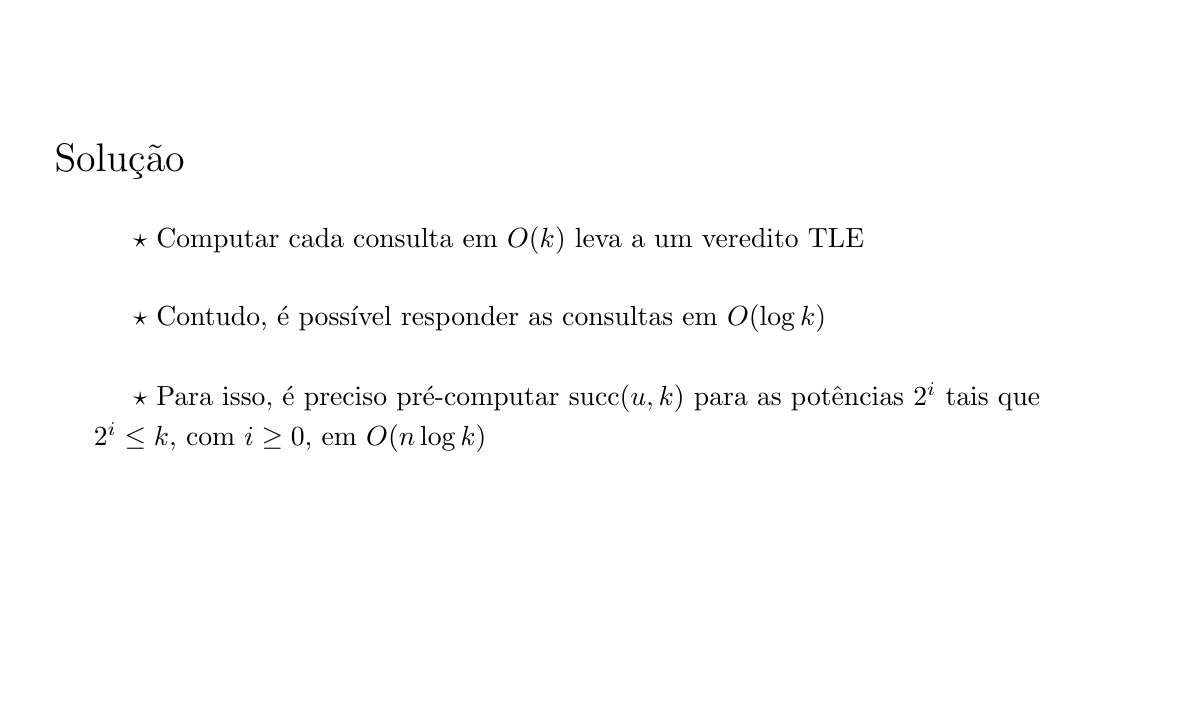
\begin{tikzpicture}
\node[draw,opacity=0] at (0, 0) {x};
\node[draw,opacity=0] at (14, 8) {x};

	\node[anchor=west] (title) at (0.0, 6.5) { \Large \bbbold{Solução} };

	\node[anchor=west] (a) at (1.0, 5.5) { $\star$ \bbtext{Computar cada consulta em $O(k)$ leva a um veredito TLE} };


	\node[anchor=west] (b) at (1.0, 4.5) { $\star$ \bbtext{Contudo, é possível responder as consultas em $O(\log k)$} };


	\node[anchor=west] (c) at (1.0, 3.5) { $\star$ \bbtext{Para isso, é preciso pré-computar $\mathrm{succ}(u, k)$ para as potências $2^i$ tais que} };

	\node[anchor=west] (c1) at (0.5, 3.0) { \bbtext{$2^i\leq k$, com $i\geq 0$, em $O(n\log k)$} };

\end{tikzpicture}
\end{frame}
\begin{frame}[plain,t]
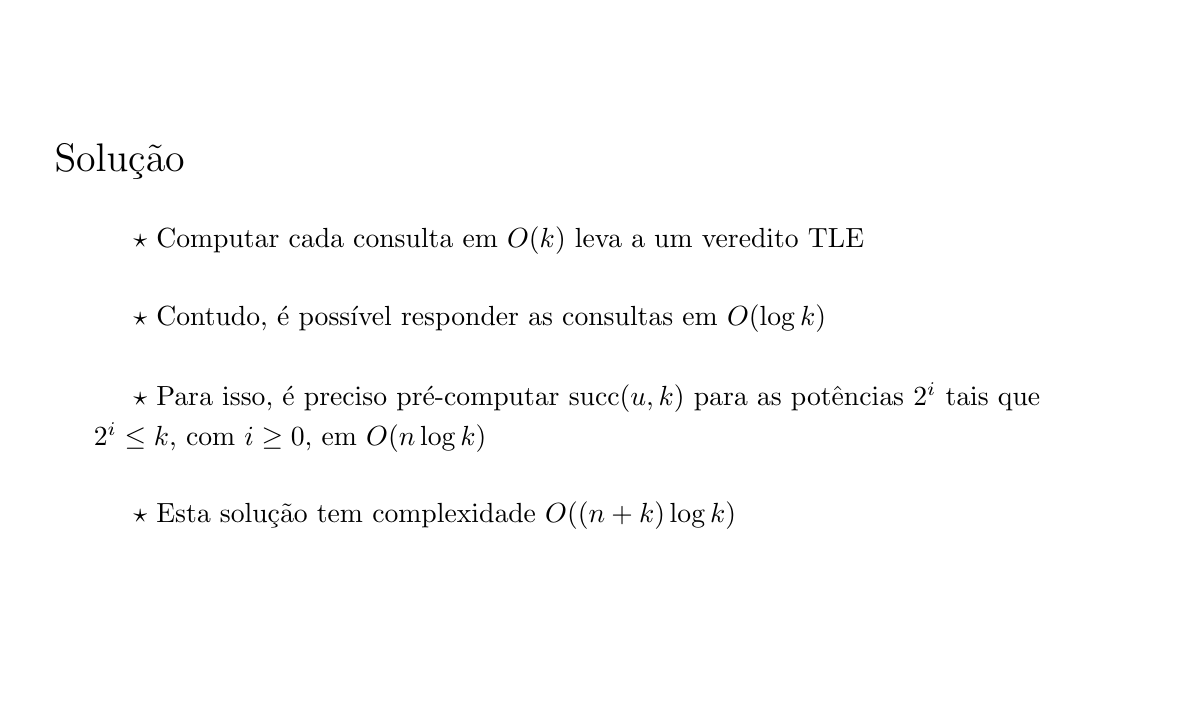
\begin{tikzpicture}
\node[draw,opacity=0] at (0, 0) {x};
\node[draw,opacity=0] at (14, 8) {x};

	\node[anchor=west] (title) at (0.0, 6.5) { \Large \bbbold{Solução} };

	\node[anchor=west] (a) at (1.0, 5.5) { $\star$ \bbtext{Computar cada consulta em $O(k)$ leva a um veredito TLE} };


	\node[anchor=west] (b) at (1.0, 4.5) { $\star$ \bbtext{Contudo, é possível responder as consultas em $O(\log k)$} };


	\node[anchor=west] (c) at (1.0, 3.5) { $\star$ \bbtext{Para isso, é preciso pré-computar $\mathrm{succ}(u, k)$ para as potências $2^i$ tais que} };

	\node[anchor=west] (c1) at (0.5, 3.0) { \bbtext{$2^i\leq k$, com $i\geq 0$, em $O(n\log k)$} };


	\node[anchor=west] (d) at (1.0, 2.0) { $\star$ \bbtext{Esta solução tem complexidade $O((n + k)\log k)$} };

\end{tikzpicture}
\end{frame}
\begin{frame}[plain,t]

\inputsnippet{cpp}{30}{40}{codes/1750.cpp}

\end{frame}
\begin{frame}[plain,t]

\inputsnippet{cpp}{11}{28}{codes/1750.cpp}

\end{frame}
\end{document}
